\documentclass[a4paper,14pt]{extarticle} %размер бумаги устанавливаем А4, шрифт 14пунктов
\usepackage[T2A]{fontenc}
\usepackage[utf8]{inputenc}

\usepackage[english,russian]{babel} %используем русский и английский языки с переносами
\usepackage{amssymb,amsfonts,amsmath,mathtext,cite,enumerate,float} %подключаем нужные пакеты расширений

\usepackage[pdftex]{graphicx, color}
\usepackage{subfigure}
\usepackage{color}
\usepackage{listings}

\usepackage{algorithm}
\usepackage{algpseudocode}

\usepackage{pdflscape}

\usepackage{longtable}

\usepackage{float}
\floatname{algorithm}{Листинг}

\DeclareGraphicsExtensions{.png,.pdf,.jpg,.mps,.bmp}
\graphicspath{{pictures/chapter1/}, {pictures/chapter2/}, {pictures/chapter3/}, {pictures/chapter4/}} %путь к рисункам
\usepackage{bmpsize}

\usepackage[nooneline]{caption} \captionsetup[table]{justification=raggedleft} \captionsetup[figure]{justification=centering,labelsep=endash}

\usepackage[left=2cm,right=2cm,top=2cm,bottom=2cm,bindingoffset=0cm]{geometry} % Меняем поля страницы

\usepackage{setspace}
\onehalfspacing % Полуторный интервал

\begin{document} 
\renewcommand{\figurename}{Рисунок}

\begin{titlepage}
\newpage

\begin{center}
Государственное образовательное учреждение высшего профессионального образования \\
\vspace{1cm}
\Large<<Московский государственный технический университет имени Н.Э. Баумана>> \\*
(МГТУ им. Н.Э. Баумана) \\*
\hrulefill
\end{center}

\flushright{ФАКУЛЬТЕТ ИНФОРМАТИКИ И СИСТЕМ УПРАВЛЕНИЯ}
\flushright{КАФЕДРА ТЕОРЕТИЧЕСКОЙ ИНФОРМАТИКИ И КОМПЬЮТЕРНЫХ ТЕХНОЛОГИЙ}

\vspace{8em}

\begin{center}
\Large Пояснительная записка \\ к дипломному проекту на тему:
\end{center}

\vspace{2.0em}

\begin{center}
	\Large
\textsc{Множественное выравнивание кодирующих последовательностей ДНК с учетом сдвигов рамки считывания}
\end{center}

\vspace{6em}

\begin{flushleft}
Студент--дипломник \hrulefill Батусов П. В. \\
\vspace{1.5em}
Научный руководитель \hrulefill Страшнов П. В.\\
\vspace{1.5em}
\end{flushleft}

\vspace{\fill}

\begin{center}
Москва 2015
\end{center}

\end{titlepage} 

\renewcommand{\baselinestretch}{1.5}

\renewcommand{\abstractname}{{Аннотация}}
%\renewcommand{\abstractname}{\Huge{Аннотация\\[1.5cm]}}
\begin{abstract}

\end{abstract}
%\clearpage

\renewcommand{\contentsname}{\centering Содержание}
\tableofcontents % это оглавление, которое генерируется автоматически

% введение
\newpage
\part*{\large \centering ВВЕДЕНИЕ}
\addcontentsline{toc}{part}{ВВЕДЕНИЕ}
\hspace{\parindent} Современная биоинформатика --- это молодая, бурно развивающаяся наука, возникшая в 1976-1978 годах и окончательно оформившаяся в 1980 году со специальным выпуском журнала <<Nucleic Acid Research>> (NAR)~\cite{MironovLect}. По сути, это собрание различных математических моделей и методов в помощь биологам для решения биологических задач, таких как: предсказание пространственной структуры белков, расшифровка структуры ДНК, хранение, поиск и аннотация биологической информации.\\
\indent Основу биоинформатики составляют сравнения. Одна из ключевых задач --- поиск сходства последовательностей. Ее решение позволяет понять функциональное назначение частей геномов, оценить эволюционное расстояние между ними. Кроме этого, различия в генотипах могут объяснить различия в фенотипах.\\
\indent Для того чтобы определить, насколько две последовательности <<похожи>>, используют алгоритмы выравнивания. Они основаны на размещении исходных последовательностей мономеров ДНК, РНК или белков друг под другом таким образом, чтобы было легко увидеть их сходные участки~\cite{WikiPairAlign}. Качество выравнивания оценивают, назначая штрафы за несовпадение букв и за наличие пробелов (когда приходится раздвигать одну последовательность для того, чтобы получить наибольшее число совпадающих позиций), например, через расстояние Левенштейна --- минимальное число элементарных операций (вставка, удаление или замена символа в строке), чтобы превратить одну строку в другую~\cite{Levenshtein}. При сравнении ищется такой вариант выравнивания, чтобы итоговый счет был максимален. В такой постановке задача называется поиском <<глобального выравнивания>>. Необходимо отметить, что для полных геномов глобальное выравнивание не работает, так как при мутации, помимо вставок, удалений и замен, бывают нелинейные перестройки, которые могут менять порядок и ориентацию целых геномных блоков. Для решения, аналогично задаче поиска глобального выравнивания, формулируют задачу поиска <<локального выравнивания>>: для двух произвольных строк $A$ и $B$ найти две самые похожие подстроки и их выравнивание.\\ 
\indent Алгоритмы множественного выравнивания, аналогично алгоритмам парного выравнивания, представляют собой инструмент для установления функциональных, структурных или эволюционных взаимосвязей между биологическими последовательностями.  Несмотря на то, что задача множественного выравнивания была сформулирована более 20 лет назад~\cite{SIAM_Journal}, она до сих пор не теряет своей актуальности. Если говорить о множественном глобальном выравнивании, то, по сравнению с парным выравниванием, практически ничего не меняется: необходимо расставить разрывы в выравниваемых строках таким образом, чтобы <<счет по столбцам>> был максимален. Счет по столбцу можно вести, перебирая все пары символов. Множественное локальное выравнивание обобщить на многомерный случай не так просто. Во-первых, какие-то подстроки могут быть не во всех последовательностях. Во-вторых, последовательности могут содержать дуплицированные участки. Поэтому для решения такой задачи необходимо более точно сформулировать условия выравнивания.\\ 
\indent Таким образом, две главные составляющие автоматических методов выравнивания --- это непосредственно алгоритм и функция оценки качества полученного результата. На сегодняшний день можно выделить два основных алгоритма выравнивания биологических последовательностей: алгоритм Нидлмана-Вунша и алгоритм Смита-Ватермана. Они представляют собой классический пример задачи динамического программирования. Существуют различные их модификации, использующие эвристики для уменьшения количества шагов алгоритма или требуемого объема памяти, однако,эти методы строят выравнивание без сохранения открытых рамок считывания. В погоне за лучшим счетом происходит потеря биологического смысла результата.\\ 
\indent Задача множественного выравнивания с учетом открытых рамок считывания требует других, более сложных подходов. Один из существующих методов решения: построить выравнивание исходной нуклеотидной последовательности на аминокислотном уровне~\cite{MACSE}. У такого подхода есть несколько проблем. Во-первых, появление преждевременного стоп-кодона. Во-вторых, так как каждая последовательность переводится с одной и той же рамкой считывания от начала и до конца, то присутствие единственного дополнительного нуклеотида приведет к аномальному переводу и выравниванию.

% глава 1
\newpage

\section[Обзор предметной области]{\large \centering Обзор предметной области}
\hspace{\parindent} Выравнивание аминокислотных или нуклеотидных последовательностей --- это процесс сопоставления сравниваемых последовательностей для такого их взаиморасположения, при котором наблюдается максимальное количество совпадений аминокислотных остатков или нуклеотидов~\cite{AlignmentClustal}. Различают два вида выравнивания: парное (выравнивание двух последовательностей ДНК, РНК или белков) и множественное (выравнивание трех и более последовательностей). 

\subsection[Существующие методы поиска гомологий в биологических последовательностях]{\large Существующие методы поиска гомологий в биологических последовательностях}
\hspace{\parindent} В генетике под гомологиями понимаются участки белков или ДНК, имеющие сходную последовательность аминокислот или нуклеотидов. Обычно существа, у которых есть гомологичные участки белков или ДНК, имеют общего предка, от которого они и получили такой участок. Поскольку в процессе эволюции ДНК подвергается мутациям, эти участки не обязательно идентичны. В них могут быть случайно заменены, добавлены или удалены нуклеотиды или аминокислоты. Некоторые мутации, такие, как транслокации и инверсии, приводят к изменениям, затрагивающим большие участки генома. Такие мутации сложно учитывать, поскольку локальное сходство проверять легче, чем глобальное, а в результате глобальных мутаций участки ДНК могут быть соединены в непредсказуемом порядке. %Поэтому существующие методы поиска гомологий умеют находить участки (подстроки) двух последовательностей, которые отличаются не очень сильно.

\subsubsection[Алгоритм Нидлмана-Вунша]{\large Алгоритм Нидлмана-Вунша}
\hspace{\parindent} Одним из наиболее распространенных алгоритмов выравнивания является алгоритм Нидлмана-Вунша~\cite{NWalgo}, основанный на двумерном динамическом программировании. Для своей работы алгоритм использует матрицу сходства, которая указывает, насколько схожими можно считать разные нуклеотиды. Использование матрицы позволяет придавать разный вес разным заменам нуклеотидов. Например, поскольку транзиции более вероятны, чем трансверсии, логично считать последовательности, отличающиеся заменой пурина на пурин или пиримидина на пиримидин, более схожими, чем те, которые отличаются заменой пурина на пиримидин или наоборот. Обычно используется симметричная матрица, однако, применение несимметричной матрицы позволяет различать замены в одну и в другую стороны. На рисунке~\ref{ris:ReplaceMatrix} представлен пример матрицы сходства. Здесь А, Г, Т и Ц обозначают, соответственно, аденин, гуанин, тимин и цитозин, а числа в матрице указывают степень сходства между двумя нуклеотидами.

\begin{figure}[h]
	\center{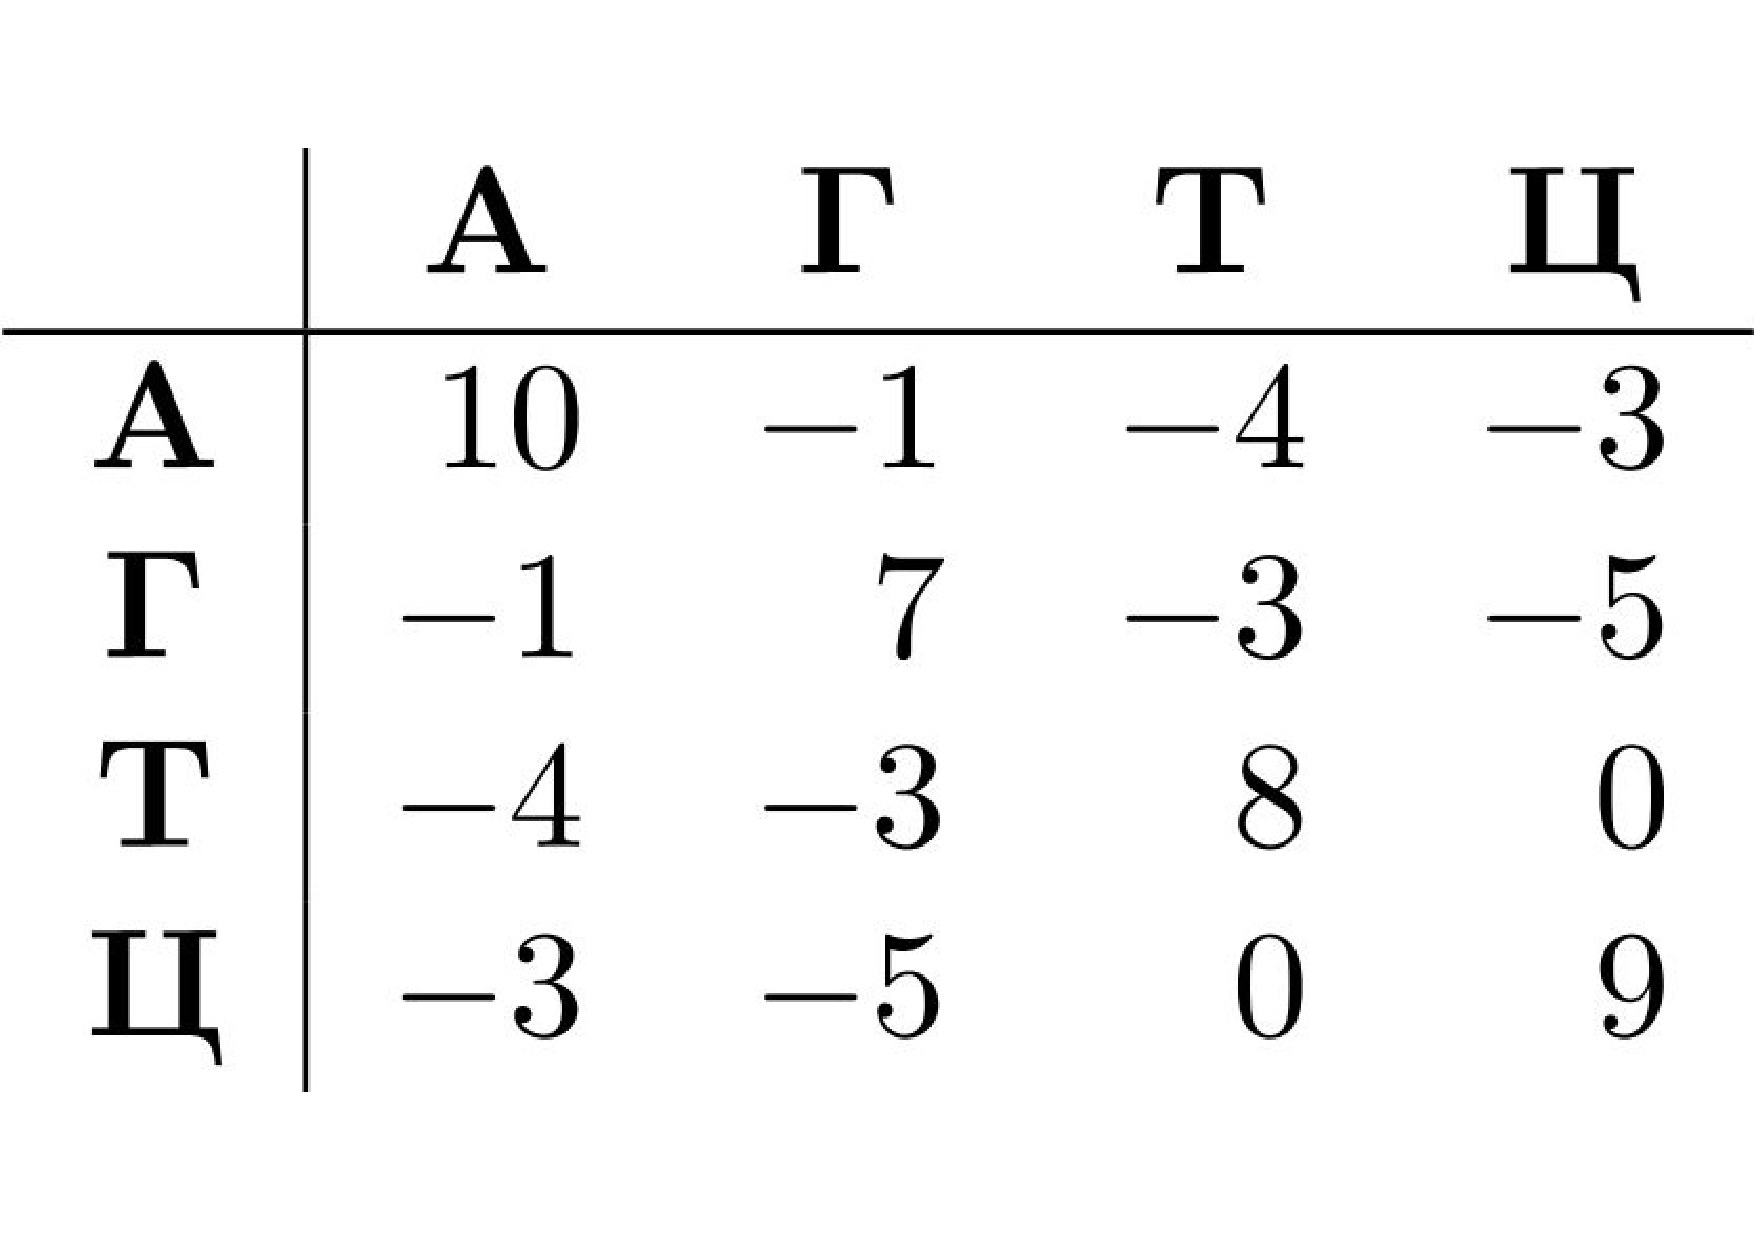
\includegraphics[width=0.4\linewidth]{RM.pdf}}
	\caption{Пример матрицы сходства}
	\label{ris:ReplaceMatrix}
\end{figure}

\indent Еще один параметр алгоритма --- штраф за разрыв последовательности. Он может выражаться произвольной функцией от длины и/или направления разрыва. Для определенности будем рассматривать линейный штраф за разрыв, определяющийся параметром $d$ (за разрыв длинны $n$ будет начислен штраф $d \cdot n$).\\
\indent На вход алгоритм получает матрицу сходства $S$, параметр штрафа $d$ и две последовательности (строки), которые необходимо выровнять. Для получения результата выполняется построение матрицы $F_{i,j}$ , где $i$ и $j$ изменяются от нуля до длины, соответственно, первой и второй строк. Вначале алгоритм инициализирует $F_{i,0}$ и $F_{0,j}$ равными, соответственно, $d \cdot i$ и $d \cdot j$ для всех $i$ и $j$. Затем происходит вычисление оставшихся элементов матрицы по формуле~\ref{eq:N_W}.

\begin{equation}\label{eq:N_W}
F_{i,j} = max\left\{
	\begin{aligned}
		& F_{i-1,j-1} + S_{A_i,B_j}\\
		& F_{i-1,j} + d\\
		& F_{i,j-1} + d
	\end{aligned}
	\right.
\end{equation}

\indent  После того, как матрица посчитана, необходимо определить, каким путем появилось значение в правом нижнем углу. Например, если $F_{i,j} = F_{i-1,j-1} +S_{A_{i-1},B_{j-1}}$, то элемент $(i, j)$ появился из элемента $(i - 1, j - 1)$, и т. д. Элементы в верхней строке произошли из элементов левее себя, элементы из левого столбца --- из элементов выше себя. Переход вида $(i, j) \rightarrow (i - 1, j - 1)$ означает, что $i$-му символу в первой строке соответствует $j$-й символ во второй строке. Переход вида $(i, j) \rightarrow (i - 1, j)$ означает, что $i$-му символу первой строки ничего не соответствует, а переход $(i, j) \rightarrow (i, j - 1)$ --- что $j$-му символу второй строки ничего не соответствует. Путь в матрице от левого верхнего угла к правому нижнему даст искомое выравнивание последовательностей.\\
\indent Очевидно, что алгоритм всегда ищет выравнивание с максимальным счетом, так как строя матрицу $F$, он рассматривает всевозможные варианты размещения одной строки относительно другой. Время работы и количество используемой памяти пропорционально произведению длин последовательностей.

\subsubsection[Алгоритм Смита-Ватермана]{\large Алгоритм Смита-Ватермана}
\hspace{\parindent} Алгоритм Смита-Ватермана~\cite{SWalgo} аналогичен алгоритму Нидлмана-Вунша, но решает задачу локального выравнивания: находит подстроки первой и второй строк, обладающие максимальным сходством.\\
\indent На вход алгоритм получает матрицу сходства $S$, две последовательности и два вектора $I$ и $D$, вектор стоимостей добавления и вектор стоимостей удаления, соответственно. Элементы матрицы $F_{i,0}$ и $F_{0,j}$ инициализируются нулями.  Вычисление оставшихся элементов происходит по формуле~\ref{eq:S_W}.

\begin{equation}\label{eq:S_W}
F_{i,j} = max\left\{
	\begin{aligned}
		& F_{i-1,j-1} + S_{A_i,B_j}\\
		& F_{i-1,j} + D_{A_i}\\
		& F_{i,j-1} + I_{B_j}\\
		& 0
	\end{aligned}
	\right.
\end{equation}

\indent Для получения выравнивания необходимо найти максимальный элемент в матрице. Если переходить от этого элемента по цепочке предыдущих, то путь закончится в каком-то нулевом элементе. Индексы этих двух элементов равны индексам начал и концов подстрок: первые индексы --- в первой строке, вторые --- во второй. Путь интерпретируется так же, как и в алгоритме Нидлмана-Вунша.\\
\indent Видно, что оба алгоритма похожи друг на друга. Они имеют одинаковую сложность и затраты по памяти, что делает такие алгоритмы неприемлемыми для работы с большим количеством генетического материала.

\subsubsection[Алгоритм Хиршберга]{\large Алгоритм Хиршберга}
\hspace{\parindent} Оба предыдущих алгоритма требуют объем памяти, пропорциональный произведению длин выравниваемых последовательностей, что затрудняет обработку больших строк, поэтому очень важно иметь методы, уменьшающие затраты памяти без критического увеличения времени счета. В 1975 году был предложен алгоритм Хиршберга, значительно сокращающий затраты памяти~\cite{Hirshberg}. Он позволяет вычислять оптимальное выравнивание строк длины $n$ и $m$, используя $O(n+m)$ количество памяти, но примерно вдвое большее времени счета по сравнению с алгоритмом Нидлмана-Вунша.\\
\indent Идея алгоритма состоит в том, что одна из двух входных последовательностей разбивается на две части, и исходная задача сводится к двум, меньшим, задачам выравнивания второй входной последовательности с каждой из частей. Решение подзадач осуществляется путем аналогичного сведения к подзадачам. На рисунке~\ref{ris:Hirshberg} показана схема разбивки задачи на две подзадачи: верхнюю, которая решается в прямоугольнике $A$ исходной таблицы, и нижнюю --- в прямоугольнике $B$. Последовательности имеют длины $n$ и $m$, соответственно. Для разбиения каждой задачи на подзадачи необходимо вычислить значение $k^*$. При этом используется объем памяти, линейно зависящий от $m$. Верхняя задача заключается в выравнивании строки с длинами не больше $n/2$ и $k^*$, а нижняя – с длинами не больше $n/2$ и $m-k^*$. 

\begin{figure}[h]
	\center{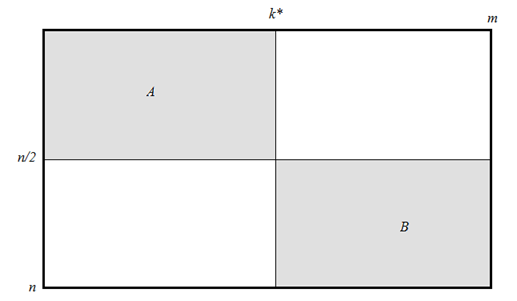
\includegraphics[width=0.7\linewidth]{hirshberg.png}}
	\caption{Разделение задачи выравнивания на две подзадачи}
	\label{ris:Hirshberg}
\end{figure}

\indent Для представления задач в алгоритме Хиршберга можно использовать бинарные деревья~\cite{HirshbergParallel}. Узлам дерева соответствуют подзадачи, которые заключаются в выравнивании меньших подпоследовательностей. Каждый узел дерева хранит в памяти границу прямоугольной области, в которой решается соответствующая задача динамического программирования. Дерево в процессе работы алгоритма строится по уровням. Сначала оно состоит только из корневого узла, который соответствует прямоугольнику $[0,0]\times[n,m]$. Создание двух узлов эквивалентно разбиению задачи на две подзадачи и разделению области решения на две, меньшего размера.\\
\indent Алгоритм Хиршберга заключается в обходе полного дерева всех подзадач. Результат выравнивания можно будет получить, если пройтись по листьям построенного дерева (рисунок~\ref{ris:HirshbergExample}). Для оптимизации вычислений можно выполнять обход (решение подзадач) только части вершин дерева: тех, которые удалены от корня на величину, не превосходящую заранее заданную константу $h$ --- максимальную глубину обхода дерева. При достижении глубины дерева $h$ или минимального размера прямоугольника применяется алгоритм Нидлмана-Вунша, который работает вдвое быстрее алгоритма Хиршберга.

\begin{figure}[h]
	\center{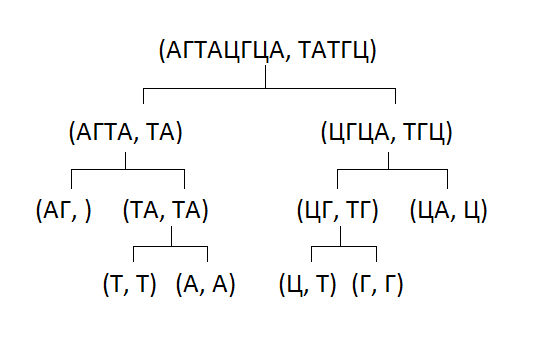
\includegraphics[width=0.7\linewidth]{hirshberg-example.png}}
	\caption{Дерево подзадач для алгоритма Хиршберга}
	\label{ris:HirshbergExample}
\end{figure}

\indent Дополнительное ускорение можно получить за счет распараллеливания. Заметим, что на каждом шаге алгоритма полученные подзадачи никак не связаны между собой, и, следовательно, их решения могут вычисляться в отдельных потоках.

\subsection[Представление генетической информации в электронном виде]{\large Представление генетической информации в электронном виде}
\hspace{\parindent} Поскольку различных нуклеотидов и стандартных аминокислот немного, для их кодирования используют один символ --- первую букву из названия. С другой стороны, названия многих аминокислот начинаются с одинаковых букв, поэтому для кодирования приходится использовать те, которые остаются незанятыми.

\subsubsection[Формат FASTA]{\large Формат FASTA}
\hspace{\parindent} В формате FASTA~\cite{FASTAformat} строчка, начинающаяся с символа '>', называется строкой описания. Она содержит имя последовательности и некоторую дополнительную информацию, предназначенную для идентификации. Другие строки, начинающиеся с символа ';', являются комментариями и игнорируются. За строкой описания следует код последовательности. При кодировании нуклеотидов буквами A, C, G, T и U кодируют, соответственно, аденин, цитозин, гуанин, тимин и урацил. Обычно, длинные последовательности разбивают на несколько строк длиной не более 80 символов --- это не правило формата, но представление данных таким образом выглядит более наглядно для человека.

\subsubsection[Формат FASTQ]{\large Формат FASTQ}
\hspace{\parindent} FASTQ --- формат представления биологической последовательности совместно с данными о качестве. Он используется для представления данных секвенирования. При кодировании уровней качества используются символы из таблицы ASCII от '!' до '\textasciitilde'.\\
\indent Существует два различных способа выражать уровень качества через вероятность ошибки: формулы~\ref{eq:FASTQ:quality1} и~\ref{eq:FASTQ:quality2}, где $Q$ --- уровень качества, а $p$ --- вероятность, что элемент последовательности ошибочный. При малых значениях $p$ эти способы дают практически идентичные результаты, но с ростом $p$ уровни качества начинают заметно различаются (рисунок~\ref{ris:FASTQscore}).

\begin{equation} \label{eq:FASTQ:quality1}
Q = -10 \cdot \log_{10} p
\end{equation}
\begin{equation} \label{eq:FASTQ:quality2}
Q = -10 \cdot \log_{10} \dfrac{p}{(1-p)}
\end{equation}
\begin{figure}[h]
	\center{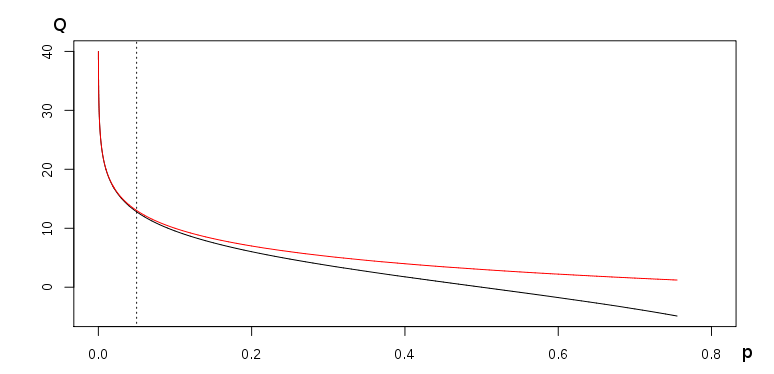
\includegraphics[width=0.9\linewidth]{FASTQscore.png}}
	\caption{График уровней качества для формул~\ref{eq:FASTQ:quality1} (красная) и~\ref{eq:FASTQ:quality2} (черная)}
	\label{ris:FASTQscore}
\end{figure}

\indent Файл в формате FASTQ содержит четыре строки для каждой последовательности. Первая строка начинается с символа '@', после которого идет описание последовательности (строка описания). Следующая строка содержит набор символов, кодирующих саму последовательность аналогично формату FASTA. За ней идёт строка, начинающаяся с символа '+', содержащая дополнительное описание последовательности. Последняя строка содержит уровни качества. 

\subsubsection[Формат GenBank]{\large Формат GenBank}
\hspace{\parindent} Запись в формате GenBank состоит из двух секций: секции аннотации и секции данных~\cite{GenBankFormat}. В первой хранится всевозможная информация о последовательности: из какого организма получена, ссылки на другие работы, различные примечания, а во второй --- сама последовательность, аналогично формату FASTA. Начало секции аннотации отмечается кодовым словом <<LOCUS>>, а секция данных начинается со слова <<ORIGIN>>. В конце описания последовательности ставится специальный маркер <<//>>. Формат GenBank, по сравнению с форматами FAST и FASTQ, позволяет представить больше дополнительной информации о последовательности.

% глава 2
\newpage

\section[Алгоритм выравнивания]{\large \centering Алгоритм выравнивания}
\hspace{\parindent} За основу был взят алгоритм Нидлмана-Вунша и произведена его модификация, благодаря которой заполнение очередной ячейки матрицы происходит с учетом трансляции текущего триплета нуклеотидов в аминокислоту. Таким образом, полученное решение строит двухуровневое выравнивание последовательностей $S_1$ и $S_2$ за время $O(len(S_1)\cdot len(S_2))$. Константа, спрятанная в оценке сложности $O$, равна 25, что позволяет продлить алгоритм до задачи множественного выравнивания.

\subsection[Принятые обозначения]{\large Принятые обозначения}
\hspace{\parindent} Пусть $S_1$ и $S_2$ --- некоторые последовательности нуклеотидов. Введем следующие обозначения:
\begin{itemize}
	\item $len(S_k)$ --- как и в предыдущих пунктах, длина последовательности $S_k$
	\item $S_k[i:j]$ --- подпоследовательность $S_k$ с $i$-го по $j$-ый нуклеотид. Запись $S_k[i:i]$, или просто $S_k[i]$, обозначает $i$-ый нуклеотид $S_k$, а в случае $j < i$ $S_k[i:j]$ является пустой последовательностью
	\item $\mathcal{A}(S_i, S_j)$ --- оптимальное выравнивание последовательностей $S_i$ и $S_j$
	\item $cost(\mathcal{A}(S_i, S_j))$ --- численная характеристика полученного выравнивания, вычисляемая по рекурсивной формуле
	\item $cost('-')$ --- штраф (число) за разрыв последовательности
	\item $cost('!')$ --- штраф за разрыв рамки считывания
	\item $cost('*')$ --- штраф за появление стоп-кодона не в конце последовательности
	\item $\sigma(X, Y)$ --- оценка за сопоставление нуклеотидов (или аминокислот) $X$ и $Y$
\end{itemize}

\indent Перепишем в новых обозначениях рекурсивную формулу $cost(\mathcal{A}(S_1, S_2))$ для классического алгоритма Нидлмана-Вунша (\ref{eq:N_W_2}).

\begin{equation}\label{eq:N_W_2}
cost(\mathcal{A}(S_1[1:i], S_2[1:j])) = max\left\{
\begin{aligned}
& cost(\mathcal{A}(S_1[1:i-1], S_2[1:j-1])) + \sigma(S_1[i], S_2[j])\\
& cost(\mathcal{A}(S_1[1:i-1], S_2[1:j])) + cost('-')\\
& cost(\mathcal{A}(S_1[1:i], S_2[1:j-1])) + cost('-')
\end{aligned}
\right.
\end{equation}

\indent На каждом шаге рекурсии происходит уменьшение $i$ и/или $j$ на единицу. Условие продолжения рекурсии: $i > 0$ и $j > 0$. Граничные значения при $i=0$ и $j=0$ заполняются по формулам~\ref{eq:N_W_gran}.
\begin{equation}\label{eq:N_W_gran}
\begin{aligned}
cost(\mathcal{A}(-, S_2[1:j])) = j\cdot cost('-')\\
cost(\mathcal{A}(S_1[1:i], -)) = i\cdot cost('-')
\end{aligned}
\end{equation}

\indent Для получения выравнивания необходимо запомнить оптимальный выбор на каждом шаге рекурсии $cost(\mathcal{A}(S_1, S_2))=cost(\mathcal{A}(S_1[1:len(S_1)], S_2[1:len(S_2)]))$ и выполнить восстановление ответа (пункт~\ref{seq:NW}).\\
\indent При построении выравнивания с учетом трансляции нуклеотидов необходимо связать уровни нуклеотидов и аминокислот. Введем дополнительную функцию $\pi(S)$, которая по входной последовательности нуклеотидов $S$ строит ее трансляцию $AA_S$. Трансляция происходит по первой рамке считывания (начиная с первого нуклеотида). Для обозначения неполных кодонов используется символ '!', а стоп-кодоны переводятся в символы '*' без остановки трансляции.\\
\indent Запишем в новых обозначениях рекурсивную формулу $cost(\mathcal{A}(S_1, S_2))$ для алгоритма двухуровневого выравнивания (\ref{eq:AA_2}), рассмотренном в пункте~\ref{NTAAalign}.

\begin{equation}\label{eq:AA_2}
cost(\mathcal{A}(S_1[1:3i], S_2[1:3j])) = max\left\{
\begin{aligned}
& cost(\mathcal{A}(S_1[1:3i-3], S_2[1:3j-3])) + \sigma(AA_1, AA_2)\\
& cost(\mathcal{A}(S_1[1:3i-3], S_2[1:j])) + cost('-')\\
& cost(\mathcal{A}(S_1[1:i], S_2[1:3j-3])) + cost('-')
\end{aligned}
\right.
\end{equation}
где $AA_1=\pi(S_1[3i-2:3i])$ и $AA_2=\pi(S_2[3j-2:3j])$\\
\indent В рассмотренных выше алгоритмах используется линейный штраф за разрыв последовательности. Для использования аффинного штрафа введем еще два параметра:
\begin{itemize}
	\item $cost(gap\_open)$ --- штраф за открытие разрыва
	\item $cost(gap\_extension)$ --- штраф за продолжение разрыва
\end{itemize}

\indent Таким образом, за разрыв длины $l$ будет начислен штраф $l\cdot cost('-')$ при линейном или $cost(gap_open) + l\cdot cost(gap_extension)$ --- при аффинном подходе.

\subsection[Построение парного выравнивания]{\large Построение парного выравнивания} \label{PairwiseAlign}
\hspace{\parindent} В отличие от алгоритма Нидлмана-Вунша, учитывающего в своей рекурсивной формуле лишь три варианта перехода (инсерция, делеция или совпадение нуклеотидов), разработанное решение рассматривает дополнительные возможности построения выравнивания с учетом образующихся аминокислот и сдвигов рамки считывания. В некоторых случаях становится выгоднее оставлять друг напротив друга различающиеся нуклеотиды, чтобы в итоге получить одинаковые аминокислоты и не допускать излишних разрывов в последовательности. Кроме этого, сигналом о построении неправильного выравнивания может служить внезапное появление стоп-кодона, на что классические алгоритмы не обращают внимания. На рисунке~\ref{ris:NWvsMULTY} показан пример двух выравниваний, построенных с помощью алгоритма Нидлмана-Вунша и собственного решения. \\
\indent Необходимо отметить, что, регулируя параметры штрафа за открытие и продолжение разрыва в последовательности, а также подобрав определенную матрицу замен нуклеотидов, можно добиться более качественного выравнивания для алгоритма Нидлмана-Вунша на этом тесте, однако, это никак не решает проблем одноуровневого подхода. Для одного набора входных данных выбранные значения будут давать хороший результат, а для другого --- нет. Постоянный подбор оптимальных параметров крайне неэффективен.

\begin{figure}[h]
	\begin{minipage}[h]{0.49\linewidth}
		\center{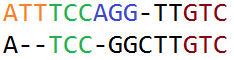
\includegraphics[width=0.8\linewidth]{NW_example} \\ а) Выравнивание по алгоритму Нидлмана-Вунша}
	\end{minipage}
	\hfill
	\begin{minipage}[h]{0.49\linewidth}
		\center{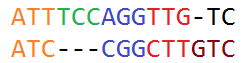
\includegraphics[width=0.8\linewidth]{multy_example} \\ б) Выравнивание по разработанному алгоритму}
	\end{minipage}
	\caption{Пример выравнивания двух последовательностей без учета аминокислотного уровня (а), и с его учетом (б). Одинаковым цветом отмечены одинаковые аминокислоты; неполные кодоны отмечены черным.}
	\label{ris:NWvsMULTY}
\end{figure}

\indent Созданный алгоритм двухуровневого выравнивания на каждом этапе выбора рассматривает все возможные варианты сопоставления от нуля до трех нуклеотидов из каждой последовательности. Таким образом, общее число возможных переходов: $\sum_{i=1}^3 2\cdot 2^i-1=25$. Для наглядности эти варианты представлены на рисунке~\ref{ris:25variants}. 

\begin{figure}[H]
	\begin{minipage}[h]{0.49\linewidth}
		\center{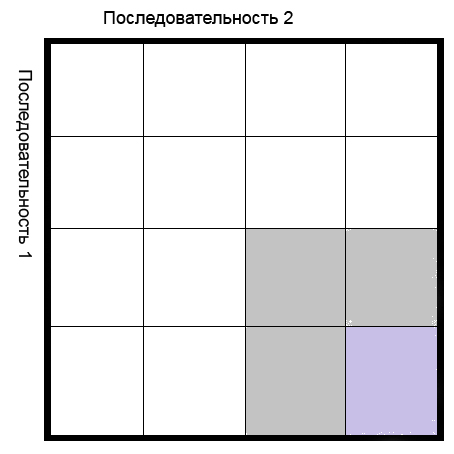
\includegraphics[width=0.65\linewidth]{NT-match} \\ а) Сопоставление нуклеотидов (3~возможных перехода)}
	\end{minipage}
	\hfill
	\begin{minipage}[h]{0.49\linewidth}
		\center{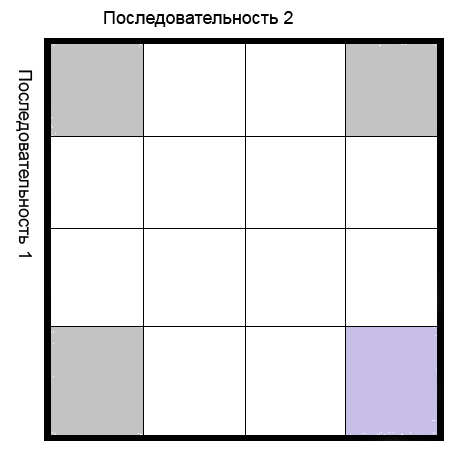
\includegraphics[width=0.65\linewidth]{AA-match} \\ б) Сопоставление аминокислот (3~возможных перехода)}
	\end{minipage}
	\vfill
	\begin{center}
		\begin{minipage}[h]{0.49\linewidth}
			\center{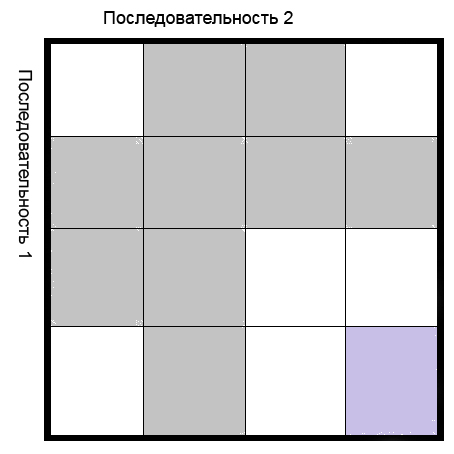
\includegraphics[width=0.65\linewidth]{frame-shift} \\ в) Сопоставление неполных кодонов (19~возможных переходов)}
		\end{minipage}
	\end{center}
	\caption{Выбор оптимального шага. Правый нижний угол таблицы представляет собой текущую позицию. Серым выделены рассматриваемые клетки для перехода.}
	\label{ris:25variants}
\end{figure}

\indent При сопоставлении неполных кодонов выходит так много вариантов, потомучто до рассматриваемых клеток перехода существует несколько возможных путей. Алгоритм учитывает их все, чтобы гарантировать оптимальное выравнивание на выходе. Ниже представлен псевдокод функции расчета $cost(\mathcal{A}(S_1, S_2))$ (листинг~\ref{lst:pairwise}).

\begin{algorithm}[H]
	\caption{Рекурсивный алгоритм построения оптимального парного выравнивания двух кодирующих последовательностей нуклеотидов} \label{lst:pairwise}
	\begin{algorithmic}
		\Procedure{$CalcAlign$}{$S_1, S_2, i, j$}
		\If{i = 0 AND j = 0} \Comment{Проверка граничных условий}
			\State \textbf{return} $0$ 
		\EndIf
		\If{i = 0 OR j = 0} 
			\State \textbf{return} $(i+j-1)*cost(gap\_extension) + cost(gap\_open)$ 
		\EndIf
		\State $AA_1 \gets \pi(S_1[i-2:i])$ \Comment{Трансляция триплетов}
		\State $AA_2 \gets \pi(S_2[j-2:j])$
		\State $stopS_1 \gets 0$
		\State $stopS_2 \gets 0$ \Comment{Проверка на появление преждевременных стоп-кодонов}
		\If{$i \neq len(S_1)$ AND $AA_1 = *$} 
			\State $stopS_1 \gets cost('*')$ 
		\EndIf
		\If{$j \neq len(S_2)$ AND $AA_2 = *$} 
			\State $stopS_2 \gets cost('*')$ 
		\EndIf \Comment{Перебор вариантов: сопоставление аминокислот}
		\State $score \gets max\left\{
		\begin{aligned}
			& CalcAlign(S_1, S_2, i-3, j-3) + \sigma(AA_1, AA_2)\\
			& CalcAlign(S_1, S_2, i-3, j) + stopS_1 + cost('-')\\
			& CalcAlign(S_1, S_2, i, j-3) + stopS_2 + cost('-')\\
		\end{aligned}
		\right.$ 
		\Statex \Comment{Перебор вариантов: сопоставление неполных триплетов}
		\State $score \gets max\left\{
		\begin{aligned}
			& CalcAlign(S_1, S_2, i-2, j-2) + \sigma(S_1[i-1], S_2[j-1]) \\ 
			& \hspace{1cm}+ \sigma(S_1[i], S_2[j]) + 2\cdot cost('!')\\
			& CalcAlign(S_1, S_2, i-2, j-1) + \sigma(S_1[i-1], S_2[j]) + 2\cdot cost('!')\\
			& CalcAlign(S_1, S_2, i-2, j-1) + \sigma(S_1[i], S_2[j]) + 2\cdot cost('!')\\
			& CalcAlign(S_1, S_2, i-2, j) + cost('!') + cost('-')\\
			& CalcAlign(S_1, S_2, i-1, j-2) + \sigma(S_1[i], S_2[j-1]) + 2\cdot cost('!')\\
			& CalcAlign(S_1, S_2, i-1, j-2) + \sigma(S_1[i], S_2[j]) + 2\cdot cost('!')\\
			& CalcAlign(S_1, S_2, i, j-2) + cost('!') + cost('-')\\
			& CalcAlign(S_1, S_2, i-3, j-2) + \sigma(S_1[i-2], S_2[j-1])\\ 
			& \hspace{1cm} + \sigma(S_1[i-1], S_2[j]) + stopS_1 + cost('!')\\
			& CalcAlign(S_1, S_2, i-3, j-2) + \sigma(S_1[i-1], S_2[j-1])\\ 
			& \hspace{1cm} + \sigma(S_1[i], S_2[j]) + stopS_1 + cost('!')\\
			& CalcAlign(S_1, S_2, i-3, j-2) + \sigma(S_1[i-2], S_2[j-1])\\ 
			& \hspace{1cm} + \sigma(S_1[i], S_2[j]) + stopS_1 + cost('!')\\
			& CalcAlign(S_1, S_2, i-3, j-1) + \sigma(S_1[i-2], S_2[j]) + stopS_1 + cost('!')\\
			& CalcAlign(S_1, S_2, i-3, j-1) + \sigma(S_1[i-1], S_2[j]) + stopS_1 + cost('!')\\
			& score
		\end{aligned}
		\right.$
		\algstore{bkbreak}
	\end{algorithmic}
\end{algorithm}

\begin{algorithm}
	\begin{algorithmic}
		\algrestore{bkbreak}
		\State $score \gets max\left\{
		\begin{aligned}	
			& CalcAlign(S_1, S_2, i-3, j-1) + \sigma(S_1[i], S_2[j]) + stopS_1 + cost('!')\\
			& CalcAlign(S_1, S_2, i-2, j-3) + \sigma(S_1[i-1], S_2[j-2])\\ 
			& \hspace{1cm} + \sigma(S_1[i], S_2[j-1]) + stopS_2 + cost('!')\\
			& CalcAlign(S_1, S_2, i-2, j-3) + \sigma(S_1[i-1], S_2[j-1])\\ 
			& \hspace{1cm} + \sigma(S_1[i], S_2[j]) + stopS_2 + cost('!')\\
			& CalcAlign(S_1, S_2, i-2, j-3) + \sigma(S_1[i-1], S_2[j-2])\\ 
			& \hspace{1cm} + \sigma(S_1[i], S_2[j]) + stopS_2 + cost('!')\\
			& CalcAlign(S_1, S_2, i-1, j-3) + \sigma(S_1[i], S_2[j-2]) + stopS_2 + cost('!')\\
			& CalcAlign(S_1, S_2, i-1, j-3) + \sigma(S_1[i], S_2[j-1]) + stopS_2 + cost('!')\\
			& CalcAlign(S_1, S_2, i-1, j-3) + \sigma(S_1[i], S_2[j]) + stopS_2 + cost('!')\\
			& score
		\end{aligned}
		\right.$
		\Statex \Comment{Перебор вариантов: сопоставление нуклеотидов}
		\State $score \gets max\left\{
		\begin{aligned}
			& CalcAlign(S_1, S_2, i-1, j-1) + \sigma(S_1[i], S_2[j]) + 2\cdot cost('!')\\
			& CalcAlign(S_1, S_2, i-1, j) + cost('!') + cost('-')\\
			& CalcAlign(S_1, S_2, i, j-1) + cost('!') + cost('-')\\
			& score\\
		\end{aligned}
		\right.$
		\State \textbf{return} $score$
		\EndProcedure
	\end{algorithmic}
\end{algorithm}

\indent Необходимо отметить, что при построении ответа нужно делать восстановление рамки в тех случаях, когда алгоритм выбрал в качестве оптимального шага сопоставление неполных триплетов (рисунок~\ref{ris:NotCompleteCodons}).

\begin{figure}[h]
	\center{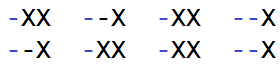
\includegraphics[width=0.6\linewidth]{not-complete-codons.png}}
	\caption{Сопоставление неполных триплетов. Цветом указаны разрывы, добавленные для сохранения текущей рамки считывания.}
	\label{ris:NotCompleteCodons}
\end{figure}

\subsection[Алгоритм кластеризации]{\large Алгоритм кластеризации}
\hspace{\parindent} Для построения множественного выравнивания используется идея выравнивания выравниваний (пункт~\ref{align-align}). Порядок объединения последовательностей определяется по методу невзвешенного попарного среднего (UPGMA --- Unweighted Pair Group Method with Arithmetic mean) \cite{legendre1998numerical}. Для использования этого алгоритма кластеризации необходимо определить функцию расстояния между выравниваемыми строками: $dist(S_i, S_j) \rightarrow \mathbb{R}$. Последовательность $S_1$ ближе к последовательности $S_2$, чем к $S_3$, если $dist(S_1, S_2) > dist(S_1, S_3)$. Чем выше значение $dist(S_i, S_j)$, тем более похожими считаются строки $S_i$~и~$S_j$.\\
\indent В качестве функции расстояния можно использовать $cost(\mathcal{A}(S_i, S_j))$, однако, ее вычисление требует больших вычислительных ресурсов. Альтернативный подход к оценке похожести двух строк --- сравнение их подстрок фиксированной длины.\\
\indent Пусть имеются две последовательности $S_1$ и $S_2$. Рассмотрим все их подстроки длины~$k$: $S_1[i: i+k-1] \in A_1, i = 1\dots len(S_1)-k+1$ и $S_2[i: i+k-1] \in A_2, i = 1\dots len(S_2)-k+1$. Расстояние между последовательностями --- это количество одинаковых подпоследовательностей $dist(S_1, S_2) = |A_1\cap A_2|$. Данный метод имеет меньшую точность, по сравнению с построением оптимального парного выравнивания, однако, он проще и требует меньше операций вычисления при небольших значениях $k$.\\
\indent На начальном этапе алгоритма кластеризации происходит вычисление расстояния между всеми последовательностями, заполняется таблица $D=dist(S_i, S_j)$ $i,j=1 \dots n$. Далее, на каждом шаге из матрицы $D$ выбирается максимальное значение, которое определяет текущие кластеры $i$ и $j$ для объединения, после чего происходит пересчет расстояний от нового кластера до всех остальных по формуле~\ref{eq:upgma} 

\begin{equation}\label{eq:upgma}
D((i,j), w)=\frac{T_iD(i,w)+T_jD(j,w)}{T_i+T_j}
\end{equation}
где $T_k$ --- количество последовательностей в кластере $k$. Старые $i$ и $j$ столбцы и строки таблицы $D$ становятся недействительными. Таким образом, с каждой новой итерацией алгоритма происходит уменьшение числа кластеров на единицу: два кластера собираются в один. Финальное объединение двух последних кластеров даст итоговое выравнивание, содержащее все исходные последовательности нуклеотидов. На рисунке~\ref{ris:UPGMA} представлен пример работы алгоритма.
\begin{figure}[h]
	\center{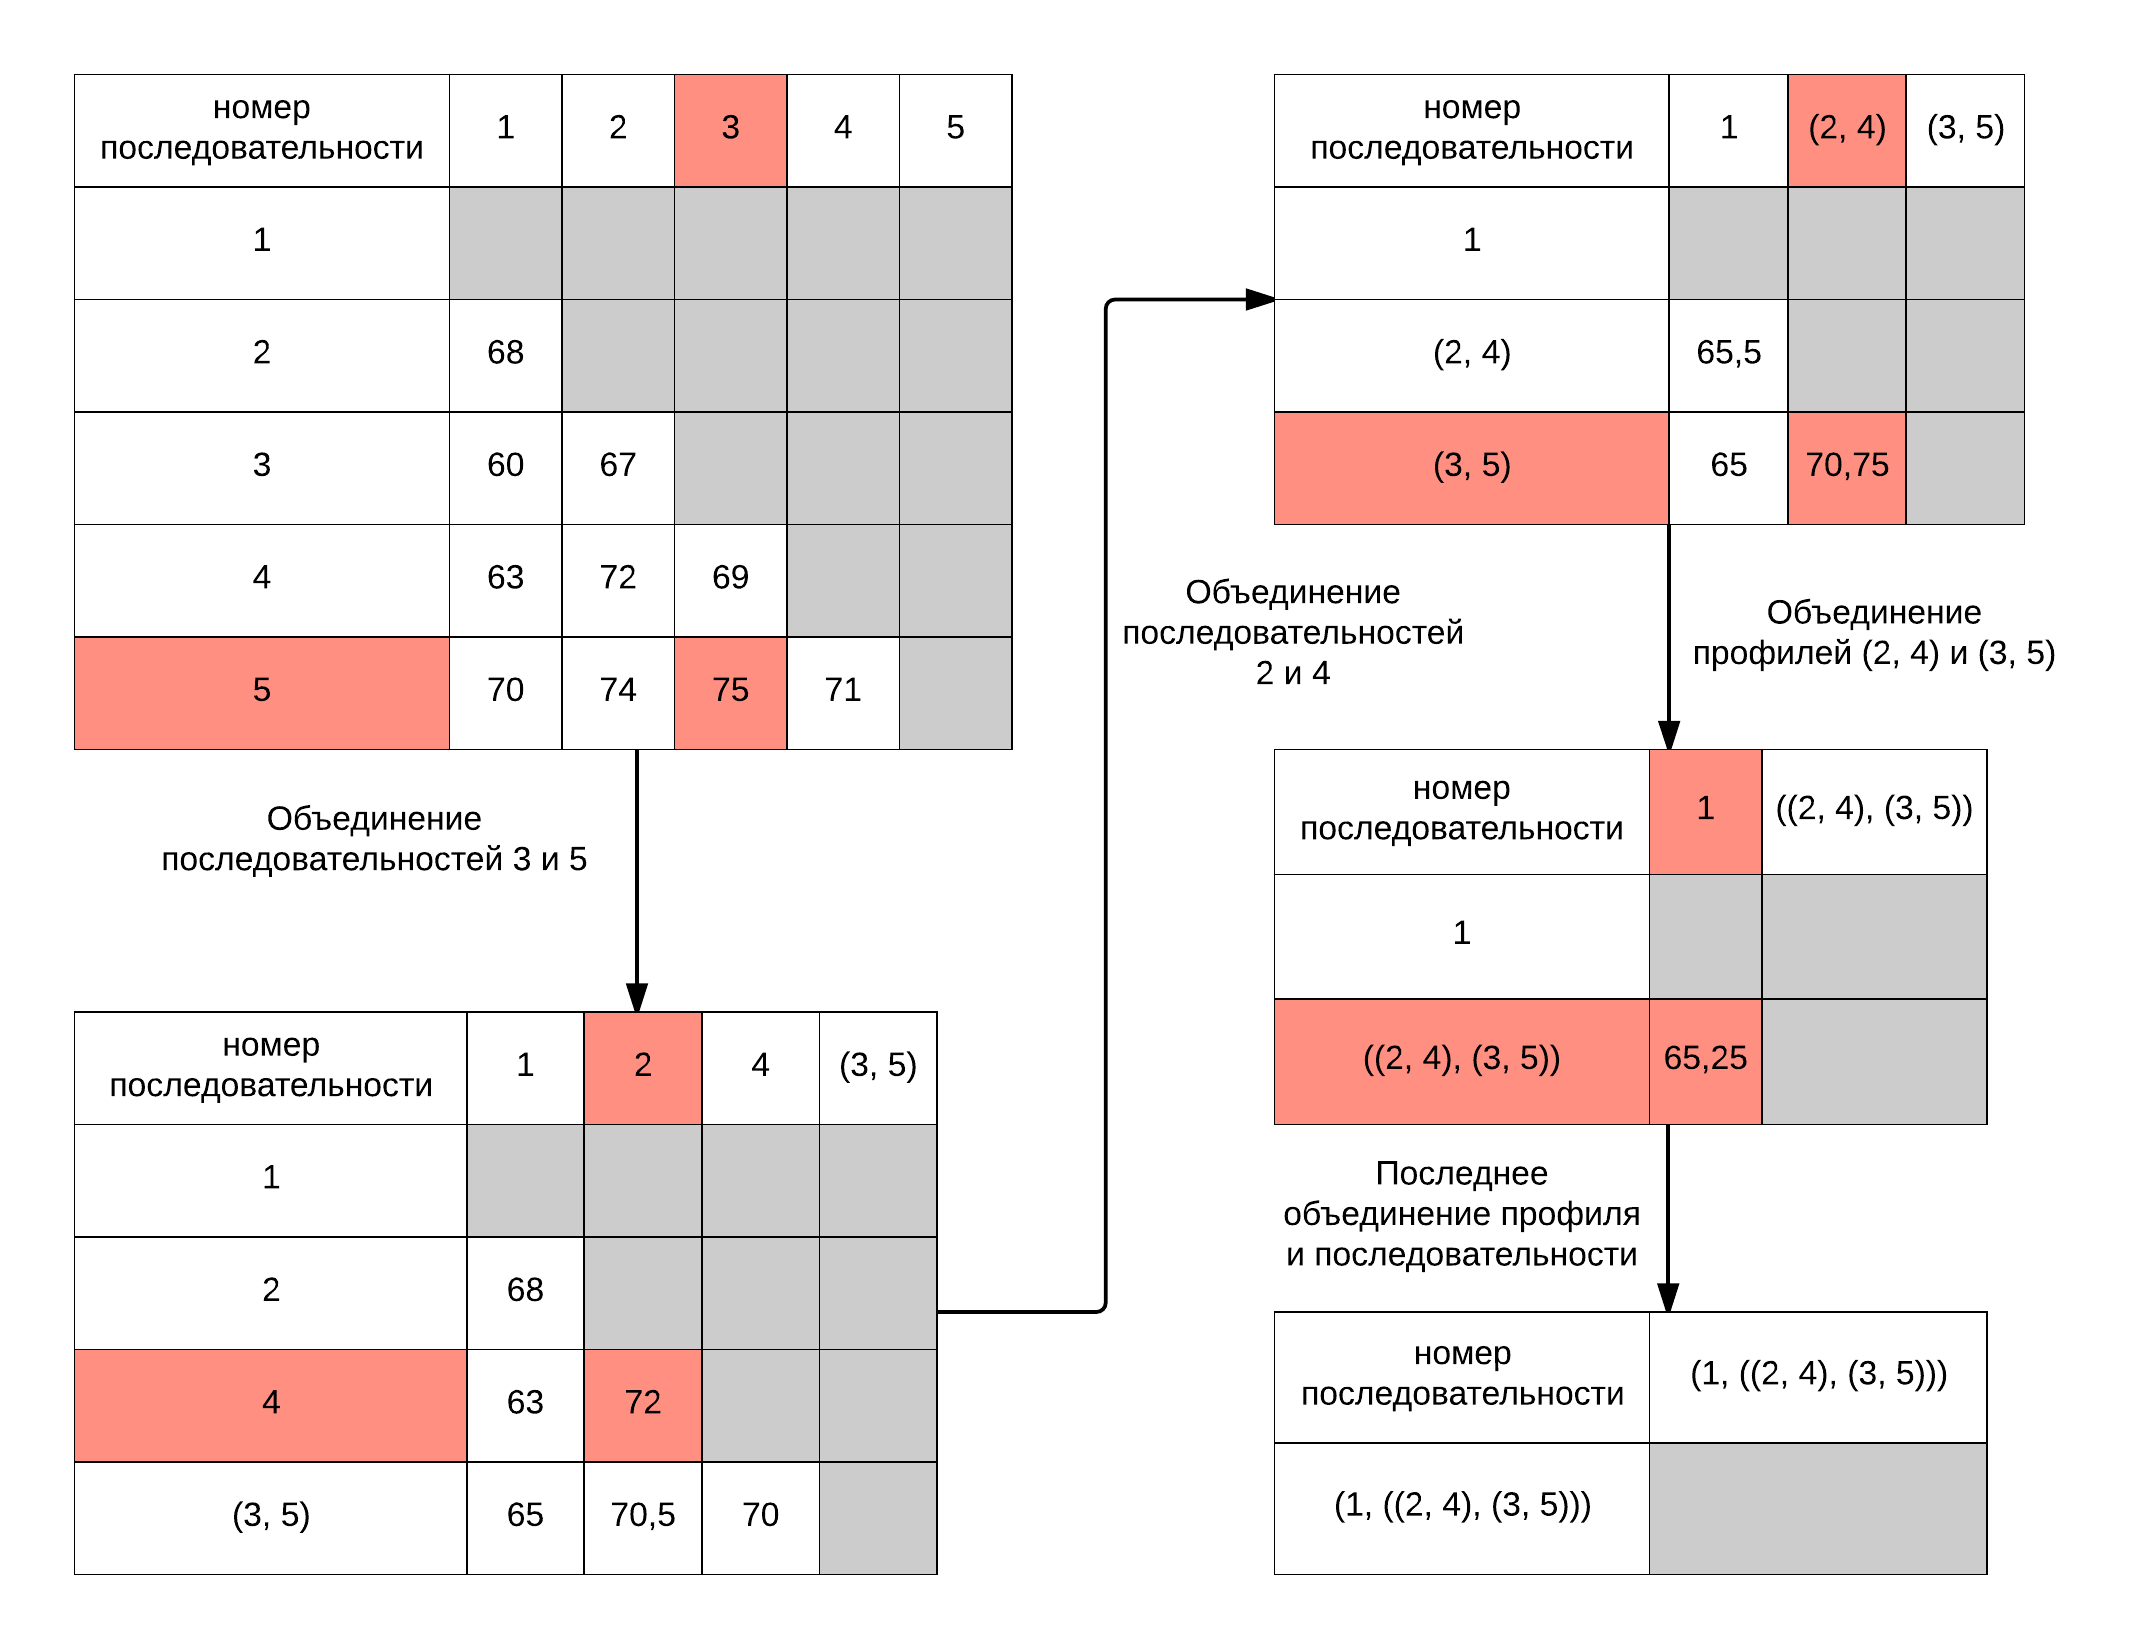
\includegraphics[width=0.85\linewidth]{UPGMA.png}}
	\caption{Изменение матрицы расстояний в процессе кластеризации. Красным цветом обозначены объединяемые кластеры.}
	\label{ris:UPGMA}
\end{figure}

\indent Необходимо отметить, что процесс кластеризации необязательно продолжать до объединения всех кластеров в один. Если найденный в таблице $D$ максимум чересчур мал, то это свидетельствует о слабом родстве последовательностей, и, чтобы не испортить построенное выравнивание, алгоритм можно остановить.

\subsection[Построение множественного выравнивания]{\large Построение множественного выравнивания}
\hspace{\parindent} Определим новое понятие <<профиль>> $P$ как набор выравненных строк. Используя рассмотренный выше алгоритм парного выравнивания, можно объединять две последовательности в один профиль $P_{12}=(\mathcal{A}(S_1, S_2)$. Для построения множественного выравнивания необходимо ввести операции сложения профилей $P_i + P_j$ и профиля со строкой $P_i + S_j$.\\
\indent При переходе от последовательностей к профилям достаточно определиться с интерпретацией $\sigma(P_1[i], P_2[j])$/$\sigma(P_1[i], S_2[j])$ и $\sigma(\pi(P_1[i-2:i]), \pi(P_2[j-2:j]))$/$\sigma(\pi(P_1[i-2:i]), \pi(S_2[j-2:j]))$, чтобы использовать алгоритм парного выравнивания для операций объединения. В отличие от строки, у профиля по $i$-ой позиции находится набор нуклеотидов из всех входящих в него последовательностей по $i$-ому индексу (рисунок~\ref{ris:profile}). Для каждого такого столбца $i=1 \dots len(P)$, где $len(P)$ --- длина профиля, можно рассчитать частоты встречающихся символов.

\begin{figure}[h]
	\center{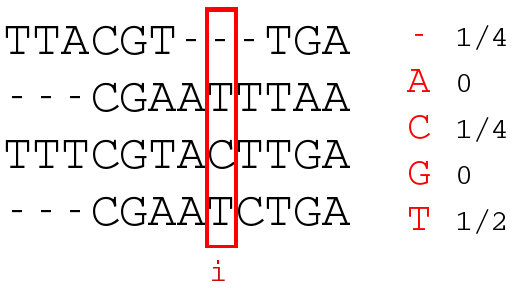
\includegraphics[width=0.6\linewidth]{profile.png}}
	\caption{Профиль из четырех последовательностей и распределение частот для $i$-го столбца}
	\label{ris:profile}
\end{figure}

Тогда, определим $\sigma(P[i], S[j])$ по формуле~\ref{eq:freq}, где $\lambda_i[N]$ --- частота нуклеотида $N$ в $i$-ом столбце профиля $P$.

\begin{equation}\label{eq:freq}
\sigma(P[i], S[j])=\sigma('A', S[j])\lambda_i['A']+\sigma('C', S[j])\lambda_i['C']+ \dots +\lambda_i['-']cost('-')
\end{equation}

Аналогичным образом вычисляется $\sigma(\pi(P[i-2:i]), \pi(S[j-2:j]))$, только в данном случае $\lambda_{i-2:i}$ содержит частоты распределения аминокислот в профиле.\\
\indent В случае объединения двух профилей необходимо рассчитать частоты для каждого из них $\lambda_i$ и $\lambda_j$, после чего произвести полный перебор по всем возможным вариантам сопоставления, как в формуле~\ref{eq:freq}. Результат вычислений нормируется, чтобы счет за сопоставление столбцов никак не зависел от количества последовательностей в профилях.\\
\indent Таким образом, итоговый алгоритм множественного выравнивания производит объединение исходных строк в профили, определяя порядок по алгоритму кластеризации. Для сложения профилей и строк используется алгоритм парного двухуровневого выравнивания.

% глава 3
\newpage

\section[Программная реализация]{\large \centering Программная реализация}
\hspace{\parindent} Разработанный алгоритм реализован на языке программирования C++ без использования сторонних библиотек и может быть запущен на всех основных операционных системах: Windows, Linux, Mac OS. Кроме основного приложения, был создан веб-интерфейс, через который также можно получить выравнивание. Так как задача требует существенных вычислительных ресурсов, практично запускать программу на мощной вычислительной платформе, а осуществлять взаимодействие с ней через веб-интерфейс. Кроме этого, для возможности внедрения отдельных компонент программы в другие проекты, были собраны статические библиотеки построения парного и множественного выравниваний.

\subsection[Структуры данных]{\large Структуры данных}
\hspace{\parindent} Ниже описанны используемые в программе структуры для хранения и обработки данных. Они также входят в состав собранных статических библиотек.

\subsubsection[Представление биологических последовательностей]{\large Представление биологических последовательностей}
\hspace{\parindent} Для представления биологических последовательностей используется структура $BioSeq$ с двумя строковыми полями:
\begin{itemize}
	\item $name$ --- идентификатор последовательности
	\item $nt\_seq$ --- последовательность нуклеотидов
\end{itemize}

Ради удобства использования у нее определен оператор индексирования [ ] и функция $Length$, возвращающая текущую длину последовательности. Чтобы иметь связь нуклеотидного и аминокислотного уровней, реализованы методы, позволяющие получить как трансляцию всей строки по первой рамке считывания, так и конкретного триплета, начинающегося с $i$-го индекса. Также, необходимо иметь возможность вставлять разрывы в последовательность, для чего были добавлены методы $InsertGap(int$ $pos)$ и $InsertGap(int$ $pos,$ $int$ $count)$, добавляющие $1$ или $count$ разрывов по индексу $pos$. Печать реализована через перегруженную операцию $<<$ (листинг~\ref{lst:BioSeqPrint}),
\begin{algorithm}
	\caption{Реализация перегруженной операции вывода $<<$ структуры BioSeq} \label{lst:BioSeqPrint}
	\begin{lstlisting}
friend std::ostream& operator << (std::ostream& stream, 
					const BioSeq& data) {
	stream << data.name << std::endl;
	stream << data.nt_seq << std::endl;
	return stream;
}
	\end{lstlisting}
\end{algorithm}

Это позволяет оформить вывод результата следующим образом: листинг~\ref{lst:BioSeqPrintExample}, однако, в качестве работы программы желательно получить выравнивание не только на нуклеотидном, но также и на аминокислотном уровне. Для наглядного разделения этих двух опций, в структуру были добавлены методы $void$ $PrintNT(std::ostream\&$ $out)$ и $void$ $PrintAA(std::ostream\&$ $out)$, которые выводят результат выравнивания и его трансляцию соответственно в указанный поток $out$.
\begin{algorithm}
	\caption{Вывод результатов выравнивания и их трансляций различными способами} \label{lst:BioSeqPrintExample}
	\begin{lstlisting}
std::vector<BioSeq*> data; 
...
for_each(data.begin(), data.end(), [] (BioSeq* seq) { 
		std::cout << *seq; 
		seq->PrintNT(std::cout);
		seq->PrintAA(std::cout);
	} );
	\end{lstlisting}
\end{algorithm}


\subsubsection[Класс построения парного выравнивания]{\large Класс построения парного выравнивания}
\hspace{\parindent} Вычисление оптимального выравнивания двух последовательностей реализовано через  класс $PairwiseAlign$. Таким образом, в одном объекте собираются и данные, и методы их обработки, что упрощает импорт алгоритма парного выравнивания в другой проект.\\
\indent Класс не содержит полей с исходными последовательностями, в нем хранятся только структуры для построения ответа и параметры выравнивания: штрафы за разрывы, смещение рамки, появление преждевременного стоп-кодона, матрицы замен нуклеотидов и аминокислот. Данные для выравнивания передаются через метод $Align(const$ $BioSeq*$ $s1,$ $const$ $BioSeq*$ $s2)$, реализующий алгоритм из пункта~\ref{PairwiseAlign}. Однако, для увеличения производительности вместо рекурсии происходит заполнение таблицы оптимальных ходов, как в классическом алгоритме Нидлмана-Вунша.

\subsubsection[Профили]{\large Профили}
\hspace{\parindent} Выравненные строки сохраняются в структуру $Profile$. Для экономии памяти и времени в профили заносятся не копии последовательностей, а только указатели на них. Функция объединения записана в виде перегруженной операции $+$ (листинг~\ref{lst:ProfilePlus}).
\begin{algorithm}
	\caption{Определение операций объединения профилей} \label{lst:ProfilePlus}
	\begin{lstlisting}
// alignment of two profiles
Profile& operator + (Profile&);
// alignment of profile and sequence
Profile& operator + (BioSeq*);
	\end{lstlisting}
\end{algorithm}

Кроме этого, профили имеют методы для вычисления оценки за сопоставление двух столбцов нуклеотидов и аминокислот. Также как и для структуры $BioSeq$ реализована возможность вставки разрывов по указанному индексу заданной длины.\\
\indent При работе с профилями необходимо гарантировать, что ни одна из входящих в его состав последовательностей не будет модифицирована или удалена до конца построения выравнивания. В противном случае, возможно появление ошибок выполнения или ухудшение качества результата. 

\subsection[Общая схема работы]{\large Общая схема работы}
\hspace{\parindent} Все разбито на отдельные блоки-этапы, блок-схема

\subsubsection[Чтение входных данных]{\large Чтение входных данных}
\hspace{\parindent} Формат входных данных, FASTA и че еще есть
как пиздато одним шмотком память выделяется
листинг с примерами, чтение FASTA

\subsubsection[Определение порядка выравниваний]{\large Определение порядка выравниваний}
\hspace{\parindent} Экономия памяти, нет перевыделения строк

\subsubsection[Объединение профилей]{\large Объединение профилей}
\hspace{\parindent} Пиздатый плюсик

\subsection[Параметры выравнивания]{\large Параметры выравнивания}
\hspace{\parindent} 

\subsection[Руководство пользователя]{\large Руководство пользователя}
\hspace{\parindent} графический интерфейс консолька

% глава 4
\clearpage
\newpage

\section[Оценка производительности]{\large \centering Оценка производительности}
\hspace{\parindent} Производительность разработанного алгоритма против существующей программы парного выравнивания MACSE оценивалась на группах синтетических тестов --- наборы созданных случайных последовательностей нуклеотидов заданной длины. Тестирование происходило на машине с процессором Intel Xeon E5645 под управлением ОС Linux Debian 7 (wheezy). Результаты тестирования представлены в таблице~\ref{tabular:results}, гистограмме (рисунок~\ref{ris:gist}) и на точечном графике (рисунок~\ref{ris:3D}).\\
\indent При тестировании были рассмотрены различные сборки разработанной программы: был использован компилятор intel icpc с различными флагами оптимизации и компилятор gcc с флагом -O3. Из графиков и таблицы хорошо видно серьезное замедление времени выполнения на больших тестах для обоих алгоритмов. Сложность полученного решения отличается от MACSE только на константу, тем не менее, был получен существенный прирост производительности.

\begin{figure}[h]
	\center{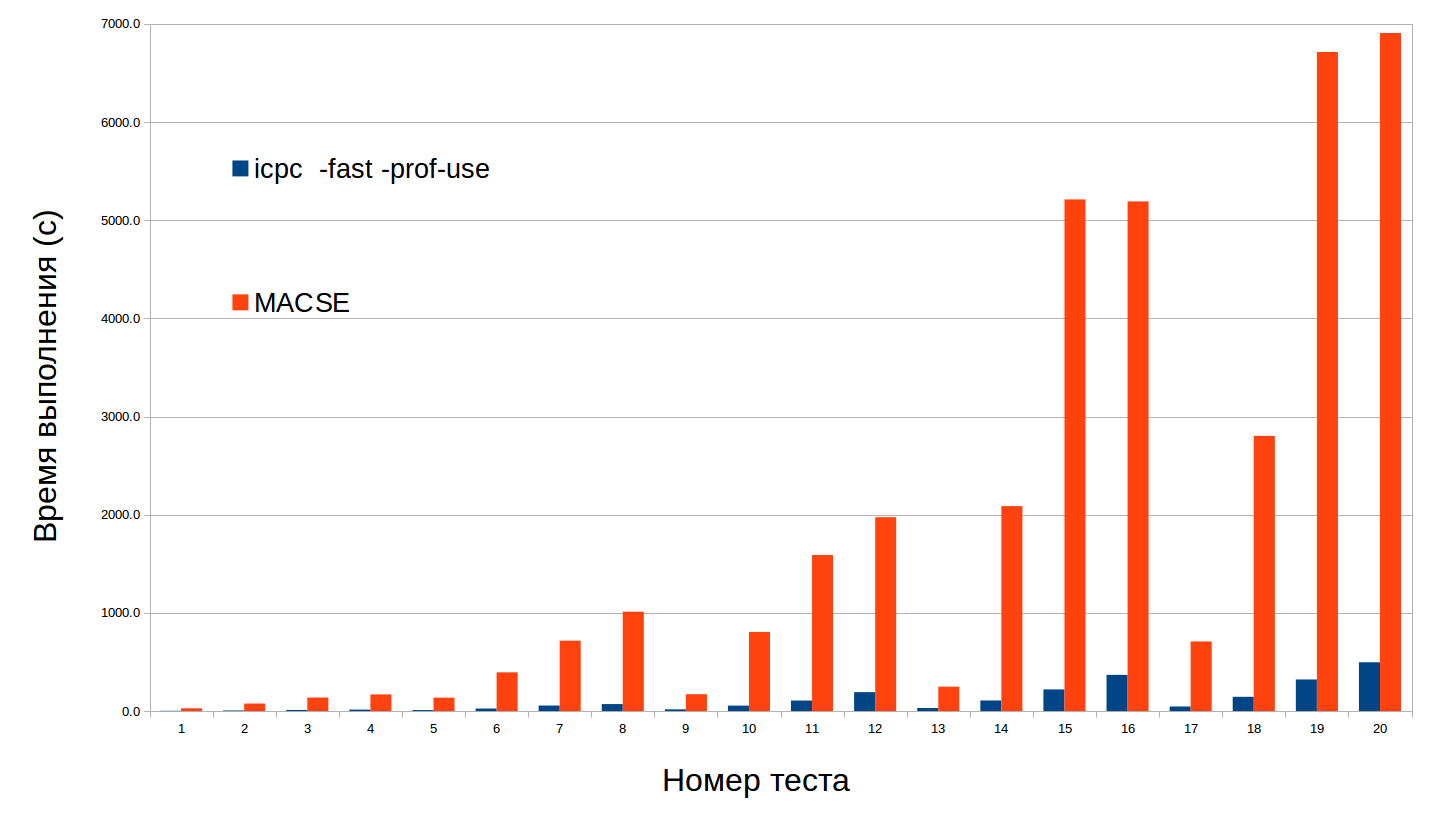
\includegraphics[width=0.65\linewidth]{gist.png}}
	\caption{Время выполнения тестов разработанного алгоритма и MACSE}
	\label{ris:gist}
\end{figure}
\begin{figure}[h]
	\center{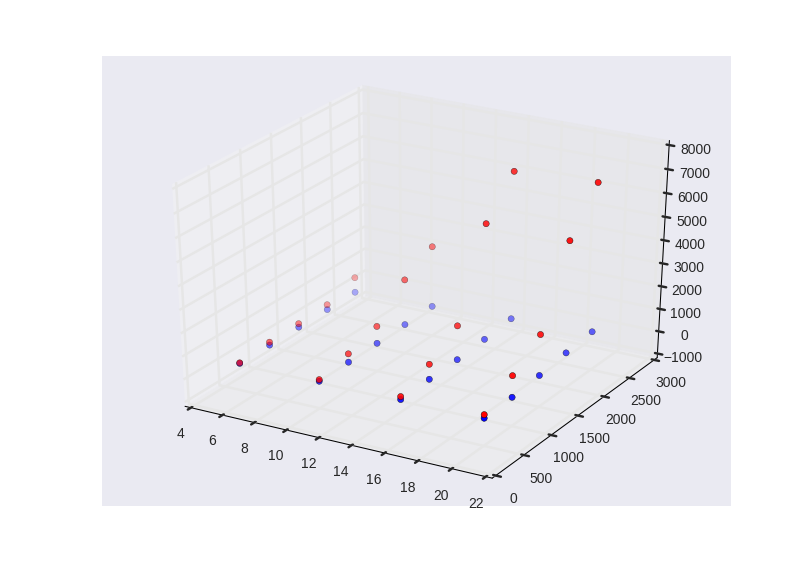
\includegraphics[width=0.65\linewidth]{3D.png}}
	\caption{График роста времени выполнения при увеличении объема входных данных}
	\label{ris:3D}
\end{figure}

\begin{landscape}
\begin{table}[htbp]
\caption{Результаты тестирования}
\begin{longtable}{|*{2}{p{3.5cm}|}*{2}{p{1.8cm}|}*{3}{p{2.8cm}|}*{2}{p{1.8cm}|}}
\hline
\multicolumn{ 1}{|p{3.5cm}|}{Длина поледовательностей} & \multicolumn{ 1}{p{3.5cm}|}{Количество последовательностей} & \multicolumn{ 7}{p{15.6cm}|}{Время выполнения (с)} \\ \cline{ 3- 9}
\multicolumn{ 1}{|p{3.5cm}|}{} & \multicolumn{ 1}{p{3.5cm}|}{} & \multicolumn{ 6}{p{10.8cm}|}{Опции компиляции } & \multicolumn{ 1}{p{1.8cm}|}{MACSE} \\ \cline{ 3- 8}
\multicolumn{ 1}{|p{3.5cm}|}{} & \multicolumn{ 1}{p{3.5cm}|}{} & \multicolumn{1}{p{1.8cm}|}{icpc -O0} & \multicolumn{1}{p{1.8cm}|}{icpc -fast} & \multicolumn{1}{p{1.8cm}|}{icpc  -fast -prof-use} & \multicolumn{1}{p{1.8cm}|}{icpc -fast -parallel} & \multicolumn{1}{p{1.8cm}|}{icpc -fast -prof-use -parallel} & \multicolumn{1}{p{1.8cm}|}{gcc -O3} & \multicolumn{ 1}{p{1.8cm}|}{} \\ \hline
500 & 5 & 11.857 & 2.364 & 2.256 & 2.344 & 2.18 & 2.832 & 27.294 \\ \hline
500 & 10 & 40.171 & 6.724 & 6.096 & 7.196 & 6.06 & 7.748 & 76.309 \\ \hline
500 & 15 & 75.969 & 12.493 & 11.409 & 11.997 & 11.097 & 14.017 & 137.789 \\ \hline
500 & 20 & 114.995 & 18.697 & 14.969 & 16.029 & 15.713 & 18.473 & 169.339 \\ \hline
1000 & 5 & 48.759 & 9.093 & 9.625 & 8.849 & 8.101 & 10.837 & 136.294 \\ \hline
1000 & 10 & 165.338 & 27.446 & 25.194 & 28.518 & 25.31 & 34.662 & 394.305 \\ \hline
1000 & 15 & 396.281 & 62.408 & 55.759 & 62.884 & 60.908 & 69.872 & 716.885 \\ \hline
1000 & 20 & 556.679 & 75.113 & 70.672 & 86.685 & 74.793 & 87.449 & 1012.063 \\ \hline
1500 & 5 & 100.462 & 18.057 & 17.009 & 18.117 & 16.553 & 22.037 & 171.643 \\ \hline
1500 & 10 & 384.48 & 60.36 & 55.371 & 65.152 & 57.016 & 78.105 & 805.822 \\ \hline
1500 & 15 & 829.996 & 117.475 & 106.651 & 115.611 & 105.979 & 135.952 & 1589.375 \\ \hline
1500 & 20 & 1551.437 & 205.153 & 192.72 & 203.841 & 196.264 & 252.428 & 1974.075 \\ \hline
2000 & 5 & 184.928 & 33.158 & 31.106 & 40.807 & 29.294 & 39.91 & 248.244 \\ \hline
2000 & 10 & 669.37 & 106.687 & 107.559 & 103.818 & 101.83 & 124.38 & 2087.51 \\ \hline
2000 & 15 & 1540.484 & 219.714 & 219.914 & 273.977 & 203.241 & 257.508 & 5212.532 \\ \hline
2000 & 20 & 2909.802 & 397.469 & 368.763 & 401.813 & 375.587 & 529.841 & 5191.924 \\ \hline
2500 & 5 & 290.254 & 53.391 & 46.495 & 50.919 & 46.239 & 62.136 & 708.756 \\ \hline
2500 & 10 & 1006.799 & 156.85 & 144.593 & 166.842 & 143.621 & 187.908 & 2803.231 \\ \hline
2500 & 15 & 2417.331 & 344.09 & 321.168 & 352.034 & 334.809 & 408.606 & 6714.268 \\ \hline
2500 & 20 & 3944.915 & 596.849 & 496.883 & 571.988 & 511.28 & 665.694 & 6907.332 \\ \hline
\end{longtable}
\label{tabular:results}
\end{table}
\end{landscape}


% заключение
\newpage
\part*{\large \centering ВЫВОДЫ}
\addcontentsline{toc}{part}{ВЫВОДЫ}
\hspace{\parindent} Целью настоящей работы являлось создание приложения для построения множественных выравниваний кодирующих последовательностей ДНК с учетом сдвигов рамки считывания. Поставленная задача была успешно выполнена, кроме этого, разработанная программа в результате тестирования показала хороший прирост скорости по сравнению с существующим аналогом. Также были созданы статические библиотеки парного и множественного выравниваний для использования в сторонних проектах. Приложение написано на языке программирования C++ и является кроссплатформенным. Для упрощения работы дополнительно к программе был создан веб-интерфейс.\\
\indent Дальнейшее развитие проекта предполагает поиск новых подходов для улучшения качества получаемого ответа. При объединении профилей, разработанный алгоритм не пересматривает предыдущие решения. Любой поставленный разрыв будет присутствовать в итоговом выравнивании. Возможно, дополнительный набор проверок и перевыравниваний сделает ответ более целым и, соответственно, более качественным.

% оглавление
\clearpage
\newpage
\bibliographystyle{utf8gost705u}  %% стилевой файл для оформления по ГОСТу
\addcontentsline{toc}{section}{\large СПИСОК ЛИТЕРАТУРЫ}
\begin{flushleft}
\bibliography{biblio}     %% имя библиографической базы (bib-файла) 
\end{flushleft}

\end{document}